\chapter{Problem statement}
Some types of cancer are suspected to either originate in or else being influenced by genetic disposition. Though human DNA has been examined and broken down to sequences of genes the meaning of most genes and their influence on each other is still unknown. The Cerberus application enables doctors to get an overview over patients' gene-expression data as well as clinical data like the history of the disease. It uses clustering techniques to provide information visualization, thereby allowing doctors to systematically search for coincidences. The aim of this thesis is to extend the application with a metabolic pathway module to take the connection between metabolic pathways and genes into account. 

\chapter{Approach}

The basic idea is to utilize preprocessed pathway and patient data to augment and/or filter the vast amount of gene-expression data for the clustering process. Using this approach it is possible to improve and refine the visualization in the gene-expression analysis and therefore provide extra information to the user. To achieve this goal the following steps need to be taken:
\begin{itemize}
\item Define a use case
\item Implement import/load functionality for pathway descriptions and provide a simple pathway editor
\item Apply graph visualization techniques to the pathway data
\item Link pathways with heatmap/dendrogram/histogram
\item Evaluate at least two multiple-display/projection techniques for presentation of the results
\end{itemize}

The block diagram in \stdref{gfx:block_diagram} shows the integration of the pathway module into the Cerberus application. The input of the clustering step is thereby taken from the gene-expression analysis.

\begin{figure}[ht]
\centering
\scalebox{0.43}{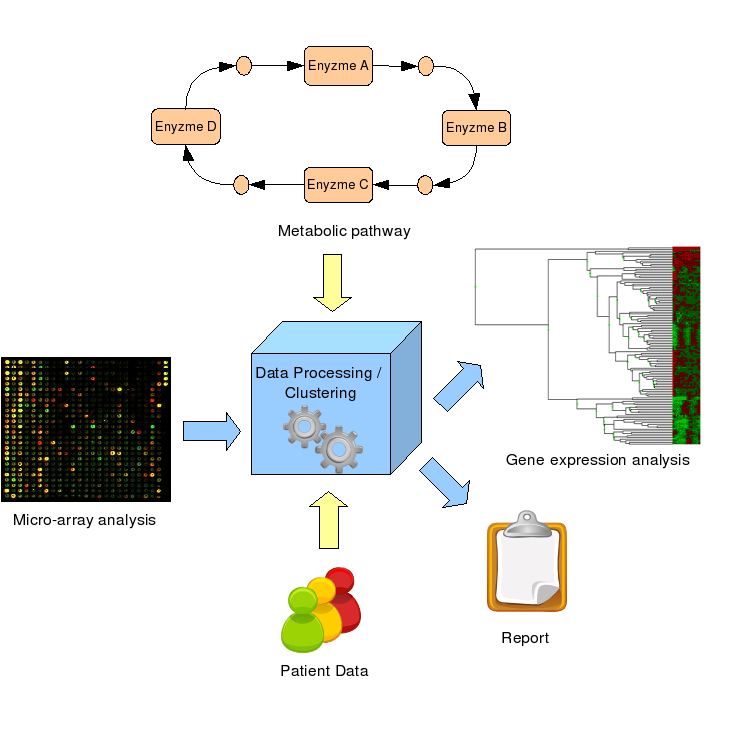
\includegraphics{gfx/block_diagram}} 
\caption[Block diagram]{\textit{Block diagram}} 
\label{gfx:block_diagram}
\end{figure}

\chapter{The tasks in detail}

\minisec{Obtain use case}

In order to visualize metabolic pathways which influence gene expression views (i.e. heatmap and dendrogram) it is of vital importance to find a use case that has medical relevance.
In collaboration with doctors and biologists a matching combination of gene data and metabolic pathways needs to be defined.

\minisec{Importing/Loading of pathway data}

The Kyoto Encyclopedia of Genes and Genomes (KEGG) \footnote{http://www.genome.jp/kegg/} Pathway Database will serve as a starting point for retrieving the initial input. Basically the pathway data can be accessed via SOAP calls over the Internet or via well structured XML files that are provided on the KEGG website. We prefer the second method because XML data can be cached locally and also stored using a Muddleware server.
The project community of KEGG is active and established a good reputation over the last years. 
However, keeping the data importing module easily extendable to fastly support further bioinformatics databases is a key issue.

\minisec{Pathway editor}

Pathways are directed graphs. With a pathway editor it should be possible for the user to alter existing imported pathways and to create simple graphs for a quick analysis. Free arranging and routing of the graph is a basic requirement. However, the focus of the work is not to build a complete graph editing and visualization tool. It rather deals with the basic functionality the user needs to proceed with the analysis (e.g. add, remove, connect and arrange graph elements).

Tentative feature list:
\begin{itemize}
\item Add nodes of different type
\item Add relations of different type
\item Rearrange and reconnecting of nodes
\item Remove nodes and relations
\item Load existing pathways
\item Import pathways from XML file
\item Switch between pathways
\item Online context information if available (provided via an integrated browser)
\item Apply and visualize external influencing factors (i.e. co-factors)
\item Apply and visualize enzyme regulation/activation
\item Apply and visualize energy level and consumption
\item Zooming
\end{itemize}

\minisec{Applying graph visualization techniques}

In a first phase only a few fundamental techniques will be supported. 
The minimum includes:
\begin{itemize}
\item Select multiple graph elements
\item Highlight either 2-step or 3-step neighborhoods
\item Highlight multiple occuring nodes
\item Partly graph highlighting (e.g. by using enzyme classes or by using users' selection)
\item Visualize flows and reaction sequences in the graph (e.g. by using Petri-Nets)
\end{itemize}

In a second phase more advanced tools could be implemented. 
For example:
\begin{itemize}
\item Visualizing several pathways in a multilayer view. The combination of basic highlighting methods with the 3D pathway layer technique potentially leads to a new innovation.
\item Semantic zoom (e.g. if pathways contain other pathways)
\end{itemize}

\minisec{Linking pathways with heatmap/dendrogram/histogram}

A major milestone of the thesis lies in the processing and visualization of the relation between pathways and gene expression data. This relation is given by enzymes which are basic elements in metabolic pathways. Enzymes are special proteins that speed up (catalyze) chemical reactions. The composition of an enzyme is encoded in a corresponding gene.

Ways to visualize these connections between pathways and genes need to be examined and applied. One possible approach is to collapse user selected pathway data and provide data information like mean, standard deviation, etc. as meta-data for the clustering process. In any case the interaction and selection process in the pathway editor must influence the gene expression visualization immediately to provide a direct feedback to the user (i.e. linking and brushing).

\minisec{Evaluation of multiple display and projection techniques}

The space consuming diagrams and the requirement of concurrent interaction in several views represent a challenge. 
A top-projection on a working desk or else a multi-monitor system 
(e.g. 4 freely arrangeable monitors) are potential candidates to boost the users' perception. 
